\chapter{Conclusion}\label{cha:conclusion}

\section{Summary}
This project has shown


This project have presented, described and compared different functional key exchange mechanisms and showed how they can be used in different scenarios. In addition to researching the concepts of \gls{abake} and \gls{ibake}and how these schemes are constructed, an actual application taking advantages of \gls{abake} are presented with models and a demonstration. The application described uses \gls{abe} as the encapsulation mechanism so that each user can provide their own contribution, thus achieving old encapsulation secrecy - assuring that a set of compromised old encapsulations will not reveal the new session key. The system provides mutual authentication since only users with the correct attributes can obtain all the required symmetric keys to compute the session key. 



\section{Further work}
The extended system would include a separate \gls{kms} which the users would register with to obtain their key. The best solution would probably be to have a separate virtual or physical server doing each task; attribute and key management, storage and distribution of keying material, broadcasting of chat messages/cipher texts. Figure \ref{fig:improved} shows how the extended system would look on a high level. Other features like being able to create your own rooms and administrate these would also be logical, and would have to be stored and handled somewhere. The prototype presented here will be a single room with a static policy.

\begin{figure}
\centering
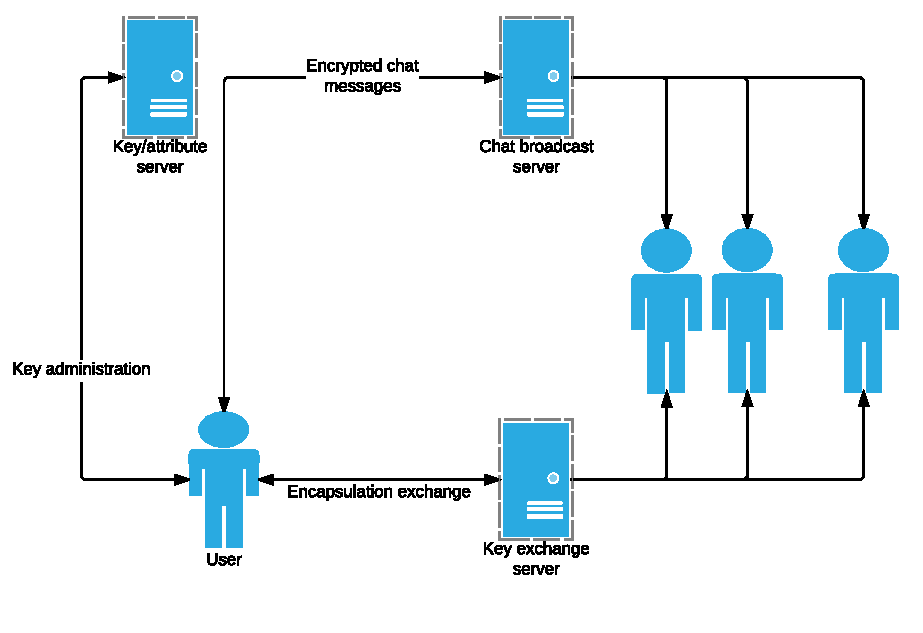
\includegraphics[trim=0cm 0cm 0cm 0cm, scale=0.8]{complete-system.pdf}
\caption{Improved system architecture}
\label{fig:improved}
\end{figure}

Another interesting extension to the system would be to remove the broadcast servers completely and apply a peer-to-peer setup, where the users distribute the encapsulations and the chat messages themself. The users would have to broadcast their encapsulations individually, the structure would look much like the one in group Diffie-Hellman as described in \ref{subsec:DH}. The users would need to have some way of knowing where to send their encapsulations, this could be solved by using multicast groups, which new users subscribes to, allowing them to receive new encapsulations, this would essentially be the same as the configuration used in this project. This setup would also require the users to negotiate the policy of the room without an intermediate server keeping track of this. To avoid pauses in the communication, the key exchange could be done in parallel while still using the old key, change to the new one when finished. 

\todo[inline]{finish this section, add reference to Scope and objectives in the introduction}
